\subsubsection{Energetic Variational Inference Approach for Machine Learning}
Variational Inference (VI) is an important research area in the field of machine learning \cite{jordan1999introduction, blei2017variational}.
Its main idea is to convert the inference problem into an optimization problem, which aims at minimizing a certain functional that measures the difference between a distribution (whose pdf is denoted by $\rho$) and the target distribution (whose pdf is denoted by $\rho^*$) over a prescribed family of distributions $\mathcal{Q}$.
For example, using the Kullback-Leibler (KL) divergence, the VI problem is formulated as the following minimization problem;
$
\rho_{\text{opt}} =\text{arg}\min_{\rho \in \mathcal{Q} }\KL(\rho||\rho^*), \text{ where } \KL( \rho ||\rho^*)  = \int \rho(\x) \ln \left( \frac{\rho(\x)}{\rho^*(\x )} \right) \dd \x.
$
Commonly, VI methods are used to approximate the posterior distribution for the Bayesian probabilistic models \cite{jordan1999introduction, neal1998view,  wainwright2008graphical, zhang2018advances}.
As alternatives to the Markov chain Monte Carlo (MCMC) sampling methods, VI methods are less computationally intensive and thus more suited to large datasets, and can be used whenever there is a need to explore many models \cite{blei2017variational}.
There have been many VI approaches developed. 
They have a very broad application in machine learning, such as VI Bayesian neural network
 \citep{grave2011practical,welling2017multiplicative, wu2019deterministic,shridhar2019comprehensive}, VI Gaussian process models \citep{king2006fast, nguyen2013efficient, nguyen2014automated, shetha2015sparse, damianou2016variational, cheng2017variational}, generative learning using VI \citep{kingma2013auto, rezende2014stochastic, goodfellow2014generative,nowozin2016f, hu2017unifying}, and many others \citep{kingma2014semi,mnih2016variational,hu2017unifying,tabak2010density}.

In the recent work of Kang and her collaborators \cite{wang2021particle}, a new VI framework named \emph{energetic variational inference} or \emph{EVI} is introduced. 
Many new EVI methods can be obtained by using different choices of divergence functional \cite{amari2012differential} and dissipation laws \cite{liu2020variational}.
These new EVI methods can also be applied to machine learning problems, including Bayesian regressions, density estimations, and generative learning, etc. 
For example, the new version of the EVI method, called ``EVI-Im'' algorithm is compared with other competing algorithms for generating samples from a star-shaped mixture Gaussian distribution as shown in Figure \ref{fig:star}. 
\begin{figure}[thbp]
\centering
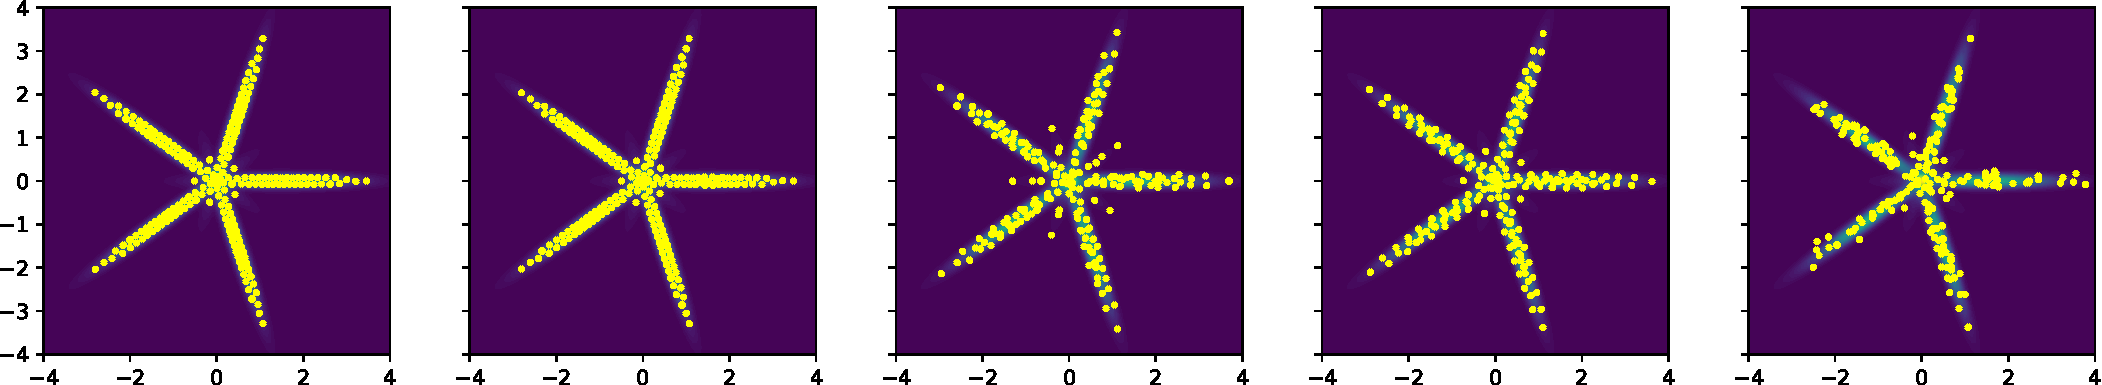
\includegraphics[width=\linewidth]{Star_compare}
\caption{ Particles obtained by various methods [200 particles]: (a) EVI-Im after 20 iterations, (b) Blob method (after 1000 iterations), (c) SVGD (after 1000 iterations), (d) matrix-valued SVGD (after 200 iterations) and (e) LMC (after 3000 iterations)}\label{fig:star}
%Particles obtained by various methods [200 particles]: EVI-Im after 20 iterations, Blob method and matrix-valued SVGD both after 1000 iterations; (b) cross-entropy v.s. number of iterations of the three methods.\label{fig:star}}
\end{figure}

The specific {\bf learning goals} for students are  to be able to
\begin{itemize}
%    \item how to program using popular software such as R, Python, or Matlab, and implement the machine learning methods covered in this project;
    \item Explain some popular machine learning tools, including Bayesian statistics, neural networks, Gaussian process models, etc. and how to use them to solve problems;
    \item Describe the above mentioned models and apply them to real-world data sets;
    \item Explain the VI concept and some popular VI methods;
    \item Implement some popular existing VI machine learning models.
\end{itemize}
The specific {\bf research goals} for students are to
\begin{itemize}
    \item Create new EVI algorithms by trying different combinations of divergence functionals and dissipation laws;
    \item Develop new numerical schemes and build software tools for implementation;
    \item Explore new applications of the EVI algorithms in machine learning focusing on supervised learning models and generative learning models to solve real-world problems based on real-world data sets. 
\end{itemize}